%! Author = Saeid Yazdani
%! Date = 7/14/2024


\section{Signal Flow for Control Loop Dynamics}
\label{sec:signal-flow-control-loop-dynamics}

Standard control theory divides linear amplifier chains into
\emph{Forward Path} (signal path from input to output) and
\emph{Feedback Path} (part of the output returns to the input).


In the forward path of an amplifier, delay and phase shift occur as the
signal passes through each stage of amplification.
These effects accumulate and affect the signal by the time it
reaches the output.

Similarly in the feedback loop, delay and phase shift are also present.
The aggregate effect of delay and phase shift in the feedback loop can affect
the stability and performance of the amplifier.
If the phase shift is large, it can cause the amplifier to become
unstable and oscillate.

The analog section of the proposed \ac{DPS} control loop includes multiple
forward and feedback paths:

\subsection*{Forward Path:}
\begin{itemize}[topsep=8pt,itemsep=4pt,partopsep=4pt, parsep=4pt]
    \item
    High-gain pre-amplifiers for low drift and high gain in a standard
    signal range (\SI{\pm10}{\volt}).
    \item
    High-voltage booster for high-voltage
    supplies (up to \SI{\pm1}{\kilo\volt}).
\end{itemize}

\subsection*{Feedback Path:}
\begin{itemize}[topsep=8pt,itemsep=4pt,partopsep=4pt, parsep=4pt]
    \item Measurement amplifiers in the current and voltage paths.
    \item Range selection components:
    \begin{itemize}
        \item Dividers for voltage detection,
        \item Current shunts or magnetic \emph{Hall Sensors},
        \item Multiplexers for range settings.
    \end{itemize}

\end{itemize}

\autoref{fig:ringing-in-multistage-loops} sketches waveform shapes when a signal
runs through a series of gain stages and faces ringing and instability which
is not acceptable for \ac{ATE} \ac{DUT} supplies.

Negative feedback is the most common configuration in such control systems for
providing better stability and control.
Each stage introduces a phase shift to the signal and these phase shifts
accumulate through multiple stages and may bring the total phase shift near
or above 180\textdegree. If the loop gain is $\ge 1$, the negative feedback will
effectively turn positive.
Other effects such as parasitic \emph{Interstage Coupling} and
\emph{Reflection} can also contribute to the total instability of the control
scheme \autocite{soo-hwan}.

\begin{figure}[!h]
    \centering
    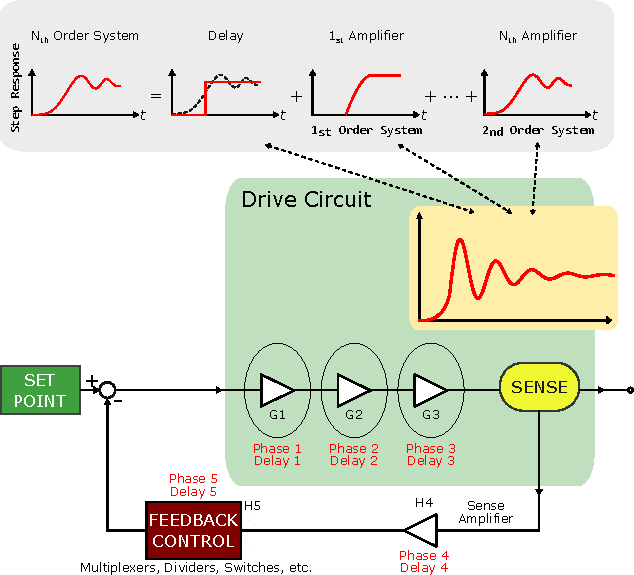
\includegraphics[width=\textwidth]
    {figures/dps_algorithms_psu/analog-loop-delay-phase-shift}
    \caption[Ringing in Multi-Stage Control Loops]{
        Signal ringing and instability induced by multiple stages in
        a power supply control loop typically contains several
        1\textsubscript{st} order stages with single reactive component (capacitor
        or inductor) for high-pass or low-pass filtering and
        2\textsubscript{nd} order stages with multiple reactive components for
        providing band-pass or band-stop filtering.
        Multiple stages may be used for noise reduction, improved
        transient response, etc.
    }
    \label{fig:ringing-in-multistage-loops}
\end{figure}

Audio amplifier developers have recognized the problem since the early
beginning of power stage design and pioneered the concept of hierarchical and
multiple feedback loops – many short feedback loops stabilize any given stage,
and the global feedback loop tries to get the best accuracy at the output
\autocite{Mikkel}.

We can adopt this approach to the \emph{Digital Domain}, and if there are
\ac{DSP} controllers we can use the methods of signal prediction:

\begin{itemize}[topsep=8pt,itemsep=4pt,partopsep=4pt, parsep=4pt]
    \item
    We know how a single stage would over-react if we knew its input and
    internal structures (gain, bandwidth, non-linearity,
    clamping behavior, etc.).

    \item
    We can \emph{calculate} compensation signals that we feed into the local
    stage’s input such that the output does not reach excessive amplitudes.

\end{itemize}

